\documentclass[10pt,conference,letterpaper]{IEEEtran}

% IEEE conference manuscript; compile with pdfLaTeX.
\usepackage{cite}
\usepackage{amsmath,amssymb,amsthm}
\usepackage{newtxtext,newtxmath}
\interdisplaylinepenalty=2500
\usepackage{booktabs}
\usepackage{array}
\usepackage{graphicx}
\usepackage{xcolor}
\usepackage{url}
\usepackage{microtype}
\usepackage[hidelinks]{hyperref}

\renewcommand{\arraystretch}{1.06}
\setcounter{dbltopnumber}{2}
\renewcommand{\dbltopfraction}{0.92}
\renewcommand{\textfraction}{0.05}
\setlength{\dblfloatsep}{2pt plus 1pt minus 1pt}
\makeatletter
\setlength{\@dblfptop}{0pt}
\setlength{\@dblfpsep}{6pt}
\setlength{\@dblfpbot}{0pt plus 1fil}
\makeatother
\newtheorem{proposition}{Proposition}
\newcommand{\method}{WLCR-SEA}
\newcommand{\routing}{structured seasonal expert routing}
\newcommand{\originalmethod}{Original WLCR-LightGBM}
\newcommand{\fixedmixture}{Fixed Seasonal Expert Mixture}
% Generated by tools/sync_rq4_evidence.py; do not edit by hand.
% manifest sha256: c8f920038d1537b32e429a3fcd32f4fe4d2d4907aad28b6e92f0a69453df24ed
% summary sha256: d17ed50074eb55013c933445b7de90fc8db725a07fb88cb00ab6135f83fc8d91
% protocol sha256: 3210382dc7bcfc7d78293178c12e1b3a850297a78d77d08e15e69b1016b127e6
\newcommand{\RQFourWLCRWAPE}{0.1967}
\newcommand{\RQFourDLinearWAPE}{0.1945}
\newcommand{\RQFourDLinearDelta}{+0.00216}
\newcommand{\RQFourDLinearCILow}{-0.00124}
\newcommand{\RQFourDLinearCIHigh}{0.00636}
\newcommand{\RQFourOriginalWAPE}{0.2002}
\newcommand{\RQFourOriginalDelta}{-0.00349}
\newcommand{\RQFourOriginalCILow}{-0.00890}
\newcommand{\RQFourOriginalCIHigh}{0.00086}
\newcommand{\RQFourPatchWAPE}{0.2171}
\newcommand{\RQFourPatchDelta}{-0.02036}
\newcommand{\RQFourPatchCILow}{-0.02679}
\newcommand{\RQFourPatchCIHigh}{-0.01439}
\newcommand{\RQFourSameHourWAPE}{0.2096}
\newcommand{\RQFourFixedMixtureWAPE}{0.2368}
\newcommand{\RQFourStandardStatWAPE}{0.2270}
\newcommand{\RQFourPriorMassPercent}{1.83}
\newcommand{\RQFourClusterCount}{727}
\newcommand{\RQFourEvaluationWindowCount}{5,110}
\newcommand{\RQFourModelSeed}{42}
\newcommand{\RQFourAugmentationSeed}{100042}
\newcommand{\RQFourWLCRBatchSize}{256}
\newcommand{\RQFourNeuralBatchSize}{128}


\title{Structured Seasonal Expert Routing for Auditable Request-Local Cellular Traffic Forecasting}
\author{\IEEEauthorblockN{Anonymous Author(s)}
\IEEEauthorblockA{Anonymous institution\\Anonymous email}}

\begin{document}
\maketitle

\begin{abstract}
Short-horizon cellular forecasting services in compartmentalized edge domains may share a global model but are prohibited from reading live traffic beyond the current target-cell request. This request-local constraint rules out predictors that require live cross-cell signals and demands a prediction path replayable from authorized evidence alone. We propose Structured Seasonal Expert Routing, instantiated as WLCR-SEA. For each 336-hour request, WLCR-SEA constructs eight named seasonal and summary experts, hard-masks unavailable ones, routes over available evidence via horizon-conditioned masked Entmax, and bounds the learned correction around the routed baseline. The finite expert interface exposes the values, masks, weights, and residuals needed to replay and inspect each prediction without accessing another cell.
On the exploratory August evaluation of 527,760 cell-hour records from 736 cells, WLCR-SEA differed from the prior traffic-only model by $+0.00045$ WAPE, with an unadjusted 95\% cell-cluster-bootstrap interval of $[-0.00312,0.00366]$, while DLinear had the lowest clean WAPE. Under matched 15\% missingness augmentation, all six selected moderate-loss intervals versus DLinear-Aug and PatchTST-Aug included zero. At the listed 50\% block, timeline-tail, and asynchronous-loss conditions, all nine differences versus the three augmentation-matched baselines were negative with unadjusted intervals below zero, conditional on five fixed corruption masks. Recorded implementation tests returned zero unavailable-expert mass, zero bounded-envelope violations, and bitwise invariance in 256 stratified request-object tests under the field allowlist. The five-seed CPU ensemble measured 34.70/38.68 ms P50/P99 under the one-thread, batch-one protocol. These findings describe an exploratory robustness--inspectability--cost profile rather than universal superiority.
The reproducible source code for WLCR-SEA has been released openly with this work.
\end{abstract}

\begin{IEEEkeywords}
cellular traffic forecasting, request-local inference, structured expert routing, sparse attention, missing telemetry, auditability
\end{IEEEkeywords}

\section{Introduction}
Short-horizon cellular-traffic forecasts support proactive radio-resource and service-capacity planning. Consider a cellular network whose operational policy allows a forecasting service to read live traffic only for the cell it is predicting. For each task, the service receives one 336-hour history window and its observation mask, and must produce a 24-hour forecast from that window alone. We call this request-local serving. In deployment, an identity-aware front end (the ingress) authorizes the request and packages the window as a sealed, self-contained input\footnote{The ingress may use the cell identifier for authorization and routing; the scorer neither receives it as a model feature nor uses it to issue identity-conditioned queries.}; the scorer combines it with a pre-provisioned global checkpoint, a shared versioned model. This arrangement creates a tension between adaptive forecasting and a prediction path that can be replayed from the evidence authorized for that request.

Our key insight is that a cellular-traffic forecast can be decomposed into a small set of named seasonal references: yesterday, last week, two weeks ago, robust medians, a trend estimate, and a prior. Each reference is either available or unavailable in a given request. Rather than leaving a black-box model to infer which references matter, we construct them explicitly, hard-mask the unavailable ones, and learn only horizon- and context-conditioned mixing weights with a bounded correction. We instantiate this design as \method{}---Window-Local Context Representation with Seasonal Expert Attention.

\begin{figure}[t]
\centering
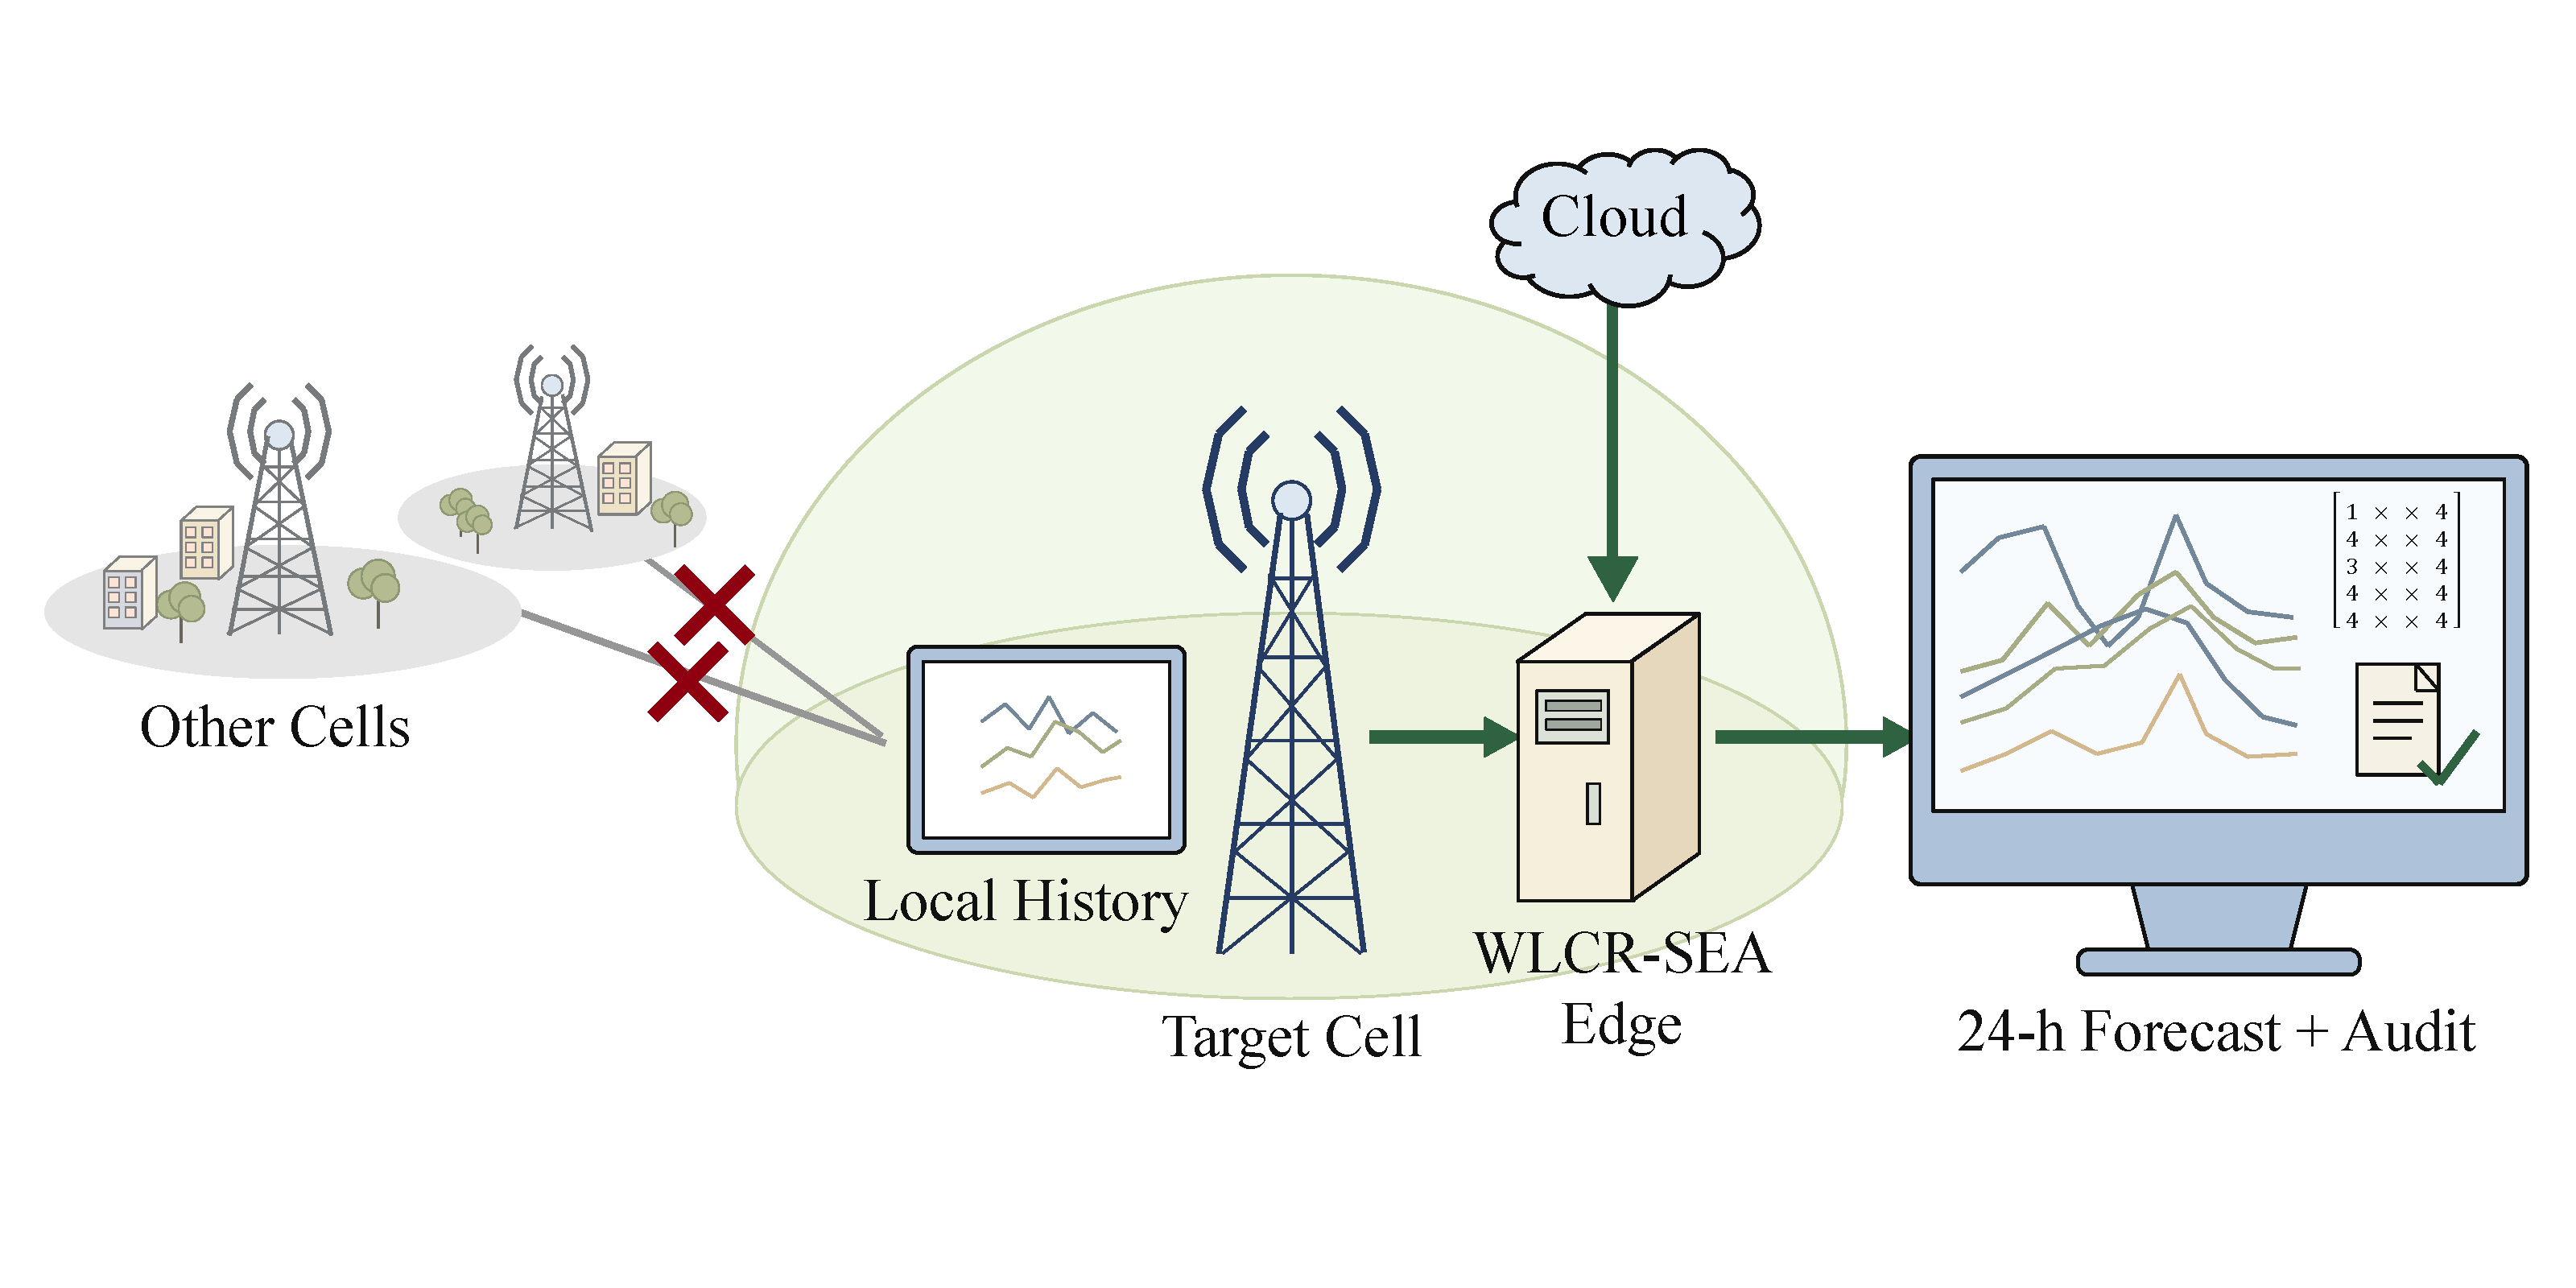
\includegraphics[width=\columnwidth,trim={80pt 70pt 180pt 50pt},clip]{figures/Scene_Diagram.pdf}
\caption{Conceptual request-local serving scenario. An ingress may use operational identity to authorize and materialize one sealed request, while the prediction process receives that request and a pre-provisioned checkpoint. The scenario delineates a self-contained online scoring path and its auditable evidence boundary.}
\label{fig:scenario}
\end{figure}

Our contributions are:
\begin{itemize}
\item We formalize a request-local serving policy and verify request-object invariance of its implemented serving path.
\item We develop \routing{} over eight named experts with horizon- and context-conditioned allocation, exact availability masking, and a bounded residual.
\item We evaluate clean accuracy, augmentation-matched missingness robustness, cell-disjoint refitting, audit properties, and same-machine latency.
\end{itemize}

We do not claim universal forecasting superiority or equivalence; we evaluate an exploratory robustness--inspectability--cost profile under the stated serving policy.


\section{Related Work}
\textbf{Spatiotemporal cellular forecasting.}
Cellular traffic exhibits temporal and spatial structure, motivating recurrent, convolutional, attention, and graph models~\cite{huang2017study,zhang2018long,wang2019spatiotemporal,zhao2022aggregation,wang2022attention,yao2023mvstgn,mehrabian2023bernstein}. Graph and multi-cell methods exploit topology and neighboring traffic to capture spatial dependence. These methods presuppose cross-cell signals at scoring time, whereas WLCR-SEA forecasts from one sealed target request.

\textbf{Request-local serving.}
Federated learning limits centralized raw-data collection while sharing model updates~\cite{zhang2021dualattention}. The present problem instead concerns the evidence available to one scoring request after an identity-aware ingress materializes a sealed input and a common checkpoint is provisioned. This deployment perspective makes request-local evidence, rather than decentralized training, the defining distinction.

\textbf{Forecasting with bounded histories and incomplete inputs.}
A global model can learn shared parameters across related series without reading other series at prediction time~\cite{montero2021global}. DLinear and PatchTST provide strong decomposition-based and patch-based baselines~\cite{zeng2023dlinear,nie2023patchtst}, while GRU-D, SAITS, and CSDI explicitly model incomplete time series~\cite{che2018grud,du2023saits,tashiro2021csdi}. Graph imputation with GRIN additionally uses inter-series structure~\cite{cini2022grin}, which is beyond the request-local serving policy studied here. Forecast combinations and dynamic model averaging also address large-scale and time-varying forecasting~\cite{makridakis2022m5,koop2012forecasting}. Unlike these predictors, WLCR-SEA exposes a finite interface of named references, availability masks, allocation weights, baseline, and residual for every forecast.

\textbf{Sparse expert routing.}
Sparse mixture-of-experts layers route computation among learned subnetworks~\cite{shazeer2017moe}, and Entmax produces normalized allocations with exact zeros~\cite{peters2019sparse}. Conventional mixtures select latent subnetworks; WLCR-SEA routes over named seasonal estimators with traceable request indices and hard availability masks. Each nonzero allocation therefore refers to a visible evidence type rather than a latent expert.

\section{Problem Formulation and Serving Access Policy}
Let $x_{c,u,q}\geq0$ denote raw hourly traffic for cell $c$, time $u$, and indicator $q\in\{1,\ldots,4\}$. In this order, the four indicators are average uplink active users, average downlink active users, average number of downlink physical resource blocks (PRBs) used, and average number of uplink PRBs used; the PRB fields are mean used-PRB counts rather than utilization ratios. The observation mask is $m_{c,u,q}\in\{0,1\}$. A request ending at hour $t$ contains
\begin{equation}
\mathcal W_{c,t}=\{(\bar{\mathbf x}_{c,u},\mathbf m_{c,u})\}_{u=t-335}^{t},
\end{equation}
where $\bar x=\log(1+x)$ for observed values. A numerical fill at a missing position is non-authoritative because every operation also receives $m$. The target is the next segment of the same four series:
\begin{equation}
\mathbf y_{c,t+h}=\mathbf x_{c,t+h},\qquad h=1,\ldots,24.
\end{equation}

All evaluated requests start at midnight. We define $t$ as the final observed 23:00 hour, so $h=1$ is the immediately following 00:00 target. A $d$-day seasonal reference uses history index
\begin{equation}
i(h,d)=335+h-24d.
\end{equation}
For $h\in[1,24]$ and $d\in[1,14]$, $i(h,d)\in[0,335]$, removing a midnight off-by-one ambiguity.

A globally fitted predictor $F_{\Theta}$ must satisfy
\begin{equation}
\widehat{\mathbf y}_{c,t+1:t+24}=F_{\Theta}(\mathcal W_{c,t})
\end{equation}
after an upstream system has materialized $\mathcal W_{c,t}$. The symbol $c$ labels the request's origin in the formulation; it is not supplied to $F_{\Theta}$ as a feature or lookup key. At prediction time, $F_{\Theta}$ cannot query traffic from $c'\neq c$, cell-specific metadata files, topology or neighbor tables, an external feature store, or a cross-request traffic cache. Frozen training statistics and globally shared checkpoint parameters $\Theta$ are allowed because they are pre-provisioned, versioned assets common to every request, not target-conditioned queries. An opaque request/origin identifier may be retained outside $F_{\Theta}$ for authorization and audit.

\begin{proposition}[Request-object serving-path invariant]
With fixed checkpoint parameters, frozen training prior, deterministic preprocessing, software state, and floating-point execution mode, two pre-extracted request-object collections containing the same target object produce identical expert tensors, routing weights, residuals, and predictions, regardless of non-target request objects.
\end{proposition}
\begin{proof}
The implemented inference field allowlist contains only the target request's \textit{x\_values}, \textit{x\_masks}, the frozen prior, and globally shared checkpoint parameters. It contains neither a cell identifier nor a client capable of performing an identity-conditioned lookup. Every subsequent tensor is a deterministic composition of these inputs under the stated execution conditions.
\end{proof}

\section{Structured Seasonal Expert Routing}
\subsection{Finite seasonal expert bank}
For compactness let $z_{u,q}=\log(1+x_{c,u,q})$. Table~\ref{tab:experts} defines eight experts for every horizon $h$ and indicator $q$. Medians use only observed values. The prior
\begin{equation}
\mu^{\mathrm{train}}_{h,q}=
\operatorname{median}_{(c,t)\in\mathcal T,\;m_{c,t+h,q}=1}
\log(1+y_{c,t+h,q})
\end{equation}
is estimated only from the applicable training layer and stored as a frozen $24\times4$ parameter.

Why these eight? Cellular traffic is dominated by daily and weekly periodicity. Experts 1--3 capture the three available seasonal lags; Experts 4--5 provide robust same-hour summaries; Expert 6 encodes a bounded weekly trend; Expert 7 is a degenerate fallback; and Expert 8 is always available. Together, these experts cover evidence types a human forecaster would inspect, making routing allocations directly inspectable as internal model behavior, but not by themselves causal explanations.

\noindent\textbf{Example.} Suppose the target hour $t+h$ is 2 PM on a Tuesday for indicator $q=1$. Expert 1 reads the observed 2 PM value on Monday, Expert 2 reads 2 PM on the previous Tuesday, and Expert 4 takes the median of the available 2 PM values from the preceding seven days. If the previous Tuesday is missing ($m_2=0$), Expert 2 is hard-masked: any prior fill is only a numerical placeholder, its routing weight is exactly zero, and the router cannot restore it through a learned allocation.

\begin{table*}[t]
\centering
\caption{Finite expert bank. $\kappa=0.5$ in the log1p domain. Unavailable values are numerically filled by the prior only for tensor safety; their mask remains zero and the hard router assigns them no mass.}
\label{tab:experts}
\footnotesize
\setlength{\tabcolsep}{4.0pt}
\begin{tabular}{c>{\raggedright\arraybackslash}p{0.19\textwidth}>{\raggedright\arraybackslash}p{0.34\textwidth}>{\raggedright\arraybackslash}p{0.30\textwidth}}
\toprule
$j$ & Expert & Log-domain value $v^{(j)}_{h,q}$ & Availability and reliability $\rho_j$\\
\midrule
1 & Last day & $z_{t+h-24,q}$ & observed point; $\rho_1=1$\\
2 & Last week & $z_{t+h-168,q}$ & observed point; $\rho_2=1$\\
3 & Two-week lag & $z_{t+h-336,q}$ & observed point; $\rho_3=1$\\
4 & Same-hour median, 7 d & $\operatorname{median}_{d=1}^{7}z_{t+h-24d,q}$ & at least one value; observed count$/7$\\
5 & Same-hour median, 14 d & $\operatorname{median}_{d=1}^{14}z_{t+h-24d,q}$ & at least one value; observed count$/14$\\
6 & Bounded weekly trend & $v^{(2)}+\operatorname{clip}(v^{(2)}-v^{(3)},-\kappa,\kappa)$ & experts 2 and 3 observed; minimum reliability\\
7 & Window-local median & $\operatorname{median}_{u=t-335}^{t}z_{u,q}$ & any observed value; observed count$/336$\\
8 & Frozen training prior & $\mu^{\mathrm{train}}_{h,q}$ & always available; $\rho_8=1$\\
\bottomrule
\end{tabular}
\end{table*}

The normalized \emph{nominal recency descriptor} is
\begin{equation}
\boldsymbol\Delta=(24,168,336,96,180,252,168,0)/336.
\end{equation}
It is a fixed expert-type descriptor under complete data, not a realized mean evidence age after request-specific missingness. The prior's zero is a type-coupled sentinel rather than an indication of recent request evidence.

The target-indicator context is
\begin{equation}
\mathbf s_{c,t,q}=[\operatorname{mean},\operatorname{median},\operatorname{sd},
r_{\mathrm{miss}},r_{\mathrm{trend}}],
\end{equation}
computed over observed log values in the request. Standard deviation is zero for a single observation. The trend is
\begin{equation}
r_{\mathrm{trend}}=
\operatorname{median}(z_{t-23:t,q})-
\operatorname{median}(z_{t-47:t-24,q}),
\end{equation}
using observed values and set to zero if either day has no observation.

\subsection{Horizon-conditioned sparse router}
For A1--A3, expert $j$ is represented without reliability,
\begin{equation}
\mathbf e^{\mathrm{A1:A3}}_j=[\mathbf e^{\mathrm{type}}_j,v_j,m_j,\Delta_j],
\end{equation}
whereas A4--A6 use
\begin{equation}
\mathbf e^{\mathrm{A4:A6}}_j=[\mathbf e^{\mathrm{type}}_j,v_j,m_j,\Delta_j,\rho_j].
\end{equation}
The query is $\mathbf q_{h,q}=g_Q([\mathbf e_h,\mathbf e_q,\mathbf s_{c,t,q}])$. For A4--A6, the score additionally contains a reliability bias,
\begin{equation}
\begin{aligned}
a_j&=\frac{\mathbf q_{h,q}^{\top}g_K(\mathbf e_j)}{\sqrt d}
+\beta\log\!\left(\max\{\rho_j,10^{-6}\}\right),\\
\beta&=\operatorname{softplus}(\widetilde\beta),
\end{aligned}
\end{equation}
and both this bias and $\mathcal L_{\mathrm{rel}}$ are absent from A1--A3.

For every hard-masked router, let $\mathcal J=\{j:m_j=1\}$. The allocation is defined on the available set,
\begin{align}
\boldsymbol\alpha_{\mathcal J}
 &=\operatorname{Entmax}_{1.5}(\{a_j:j\in\mathcal J\}),\\
\alpha_j&=0,\qquad j\notin\mathcal J .
\end{align}
The implementation compacts each available subset, applies Entmax on that subset, and scatters the result back to the eight-expert axis; it does not use a finite negative score as an exclusion surrogate. Thus unavailable experts have structurally exact zero mass. In A1 and A2, an unavailable expert retains its prior-filled value and an availability token $m_j=0$, but routing is nevertheless computed over all eight logits and may assign it nonzero mass. Entmax in A2 may be sparse, but does not structurally guarantee zero mass. A3 replaces this learned response with structural exclusion.

The learned static controls use the same available-set convention:
\begin{align}
\boldsymbol\alpha_{q,\mathcal J}&=\operatorname{softmax}(\{\theta_{q,j}:j\in\mathcal J\}), &&32\text{ parameters},\\
\boldsymbol\alpha_{h,q,\mathcal J}&=\operatorname{softmax}(\{\theta_{h,q,j}:j\in\mathcal J\}), &&768\text{ parameters},
\end{align}
with zero mass outside $\mathcal J$. The \emph{\fixedmixture{}} uses weights $(0,0.7,0.2,0.1,0,0,0,0)$, removes unavailable experts, and renormalizes; if the remaining fixed mass is zero, it falls back to the prior. This deterministic baseline is distinct from \originalmethod{}.

\begin{table}[t]
\centering
\caption{Router variants. Reliability includes its token, score bias, and auxiliary loss. \method{} denotes variant A6 outside this ablation table.}
\label{tab:variants}
\footnotesize
\setlength{\tabcolsep}{2.0pt}
\renewcommand{\arraystretch}{1.05}
\begin{tabular*}{\columnwidth}{@{\extracolsep{\fill}}clcccc@{}}
\toprule
ID & Router & \shortstack{Hard\\mask} & Reliability & \shortstack{Bounded\\residual} & \shortstack{Mixed 15\%\\augmentation}\\
\midrule
A1 & Softmax & no & no & no & no\\
A2 & Entmax$_{1.5}$ & no & no & no & no\\
A3 & Entmax$_{1.5}$ & yes & no & no & no\\
A4 & Entmax$_{1.5}$ & yes & yes & no & no\\
A5 & Entmax$_{1.5}$ & yes & yes & yes & no\\
A6 & Entmax$_{1.5}$ & yes & yes & yes & yes\\
\bottomrule
\end{tabular*}
\end{table}

\subsection{Bounded latent audit envelope}
The dynamic baseline and entropy are
\begin{align}
b_{c,t,h,q}&=\sum_{j=1}^{8}\alpha_{c,t,h,q,j}v^{(j)}_{c,t,h,q},\\
H(\boldsymbol\alpha)&=-\sum_j\alpha_j\log(\alpha_j+10^{-12}).
\end{align}
A small network receives $b$, local context, horizon and indicator embeddings, and $H$. It produces
\begin{align}
\delta&=\delta_{\max}\tanh g_R(b,\mathbf s,\mathbf e_h,\mathbf e_q,H),\\
\widehat\ell&=b+\delta,\qquad
\widehat y=\max\{10^{-4},\exp(\widehat\ell)-1\}.
\end{align}
Candidate bounds are $\delta_{\max}\in\{0.25,0.5\}$ in unnormalized log1p units and are selected on the inner layer. The convex variant sets $\delta_{\max}=0$.

\begin{proposition}[Bounded latent audit envelope]
Let $\mathcal J=\{j:m_j=1\}$. Because the prior is always available, the pre-floor latent prediction satisfies
\begin{equation}
\min_{j\in\mathcal J}v_j-\delta_{\max}
\leq \widehat\ell \leq
\max_{j\in\mathcal J}v_j+\delta_{\max}.
\end{equation}
Consequently, the final raw prediction lies in
\begin{equation}
\left[\max\{10^{-4},e^{v_{\min}-\delta_{\max}}-1\},
\max\{10^{-4},e^{v_{\max}+\delta_{\max}}-1\}\right],
\end{equation}
where $v_{\min}$ and $v_{\max}$ are the minimum and maximum values on $\mathcal J$.
\end{proposition}
\begin{proof}
For a hard-masked variant, the dynamic baseline is a convex combination of available expert values and therefore lies in their convex hull. Adding a residual whose absolute value is at most $\delta_{\max}$ gives the latent bounds. Monotonicity of the exponential and the final non-negativity floor gives the raw-domain interval.
\end{proof}

\subsection{Training, augmentation, and request record}
WLCR-SEA keeps its experts, prior, residual, and masked L1 objective in the \emph{unnormalized} log1p domain. For observed targets it minimizes
\begin{equation}
\mathcal L=\mathcal L_{\mathrm{pred}}
+10^{-3}\mathcal L_{\mathrm{res}}
+\lambda_{\mathrm{rel}}\mathcal L_{\mathrm{rel}},
\end{equation}
where $\mathcal L_{\mathrm{pred}}$ is masked L1 between unnormalized log1p prediction and target, $\mathcal L_{\mathrm{res}}=\operatorname{mean}(\delta^2)$, and $\mathcal L_{\mathrm{rel}}=\operatorname{mean}_j[\alpha_j(1-\rho_j)]$. We set $\lambda_{\mathrm{rel}}=10^{-3}$ only for A4--A6 and exactly zero for A1--A3.

For \method{} (A6), each fit or final-training stage and each data/model seed receives one deterministic 15\% input-history view, held fixed for all epochs. A stable hash selects one of MCAR, block, timeline-tail, or asynchronous loss uniformly for each cell. MCAR, block, and timeline-tail masks are synchronous across indicators; asynchronous masks are independent by indicator. Masks are generated on unique cell--time keys before window extraction and then projected into overlapping requests. Labels and target masks are unchanged. For the fair robustness comparison, \method{}, DLinear-Aug, PatchTST-Aug, and GRU-D-Direct-Aug call the same deterministic mask generator with the same data seed and therefore receive the same pre-generated view; the final stage uses seed $s+100000$ for model seed $s$.

The serving computation exposes core fields for a proposed fixed-schema semantic audit record:
\begin{equation}
\mathcal A_{c,t,h,q}=
\{\alpha_j,v_j,m_j,\rho_j\}_{j=1}^{8}
\cup\{b,\delta,H,|\operatorname{supp}(\alpha)|\}.
\end{equation}
A deployable record would additionally carry schema, checkpoint-hash, and transform-version identifiers; its serialization is outside the reported latency benchmark. Figure~\ref{fig:architecture} summarizes the request path.

\begin{figure*}[t]
\centering
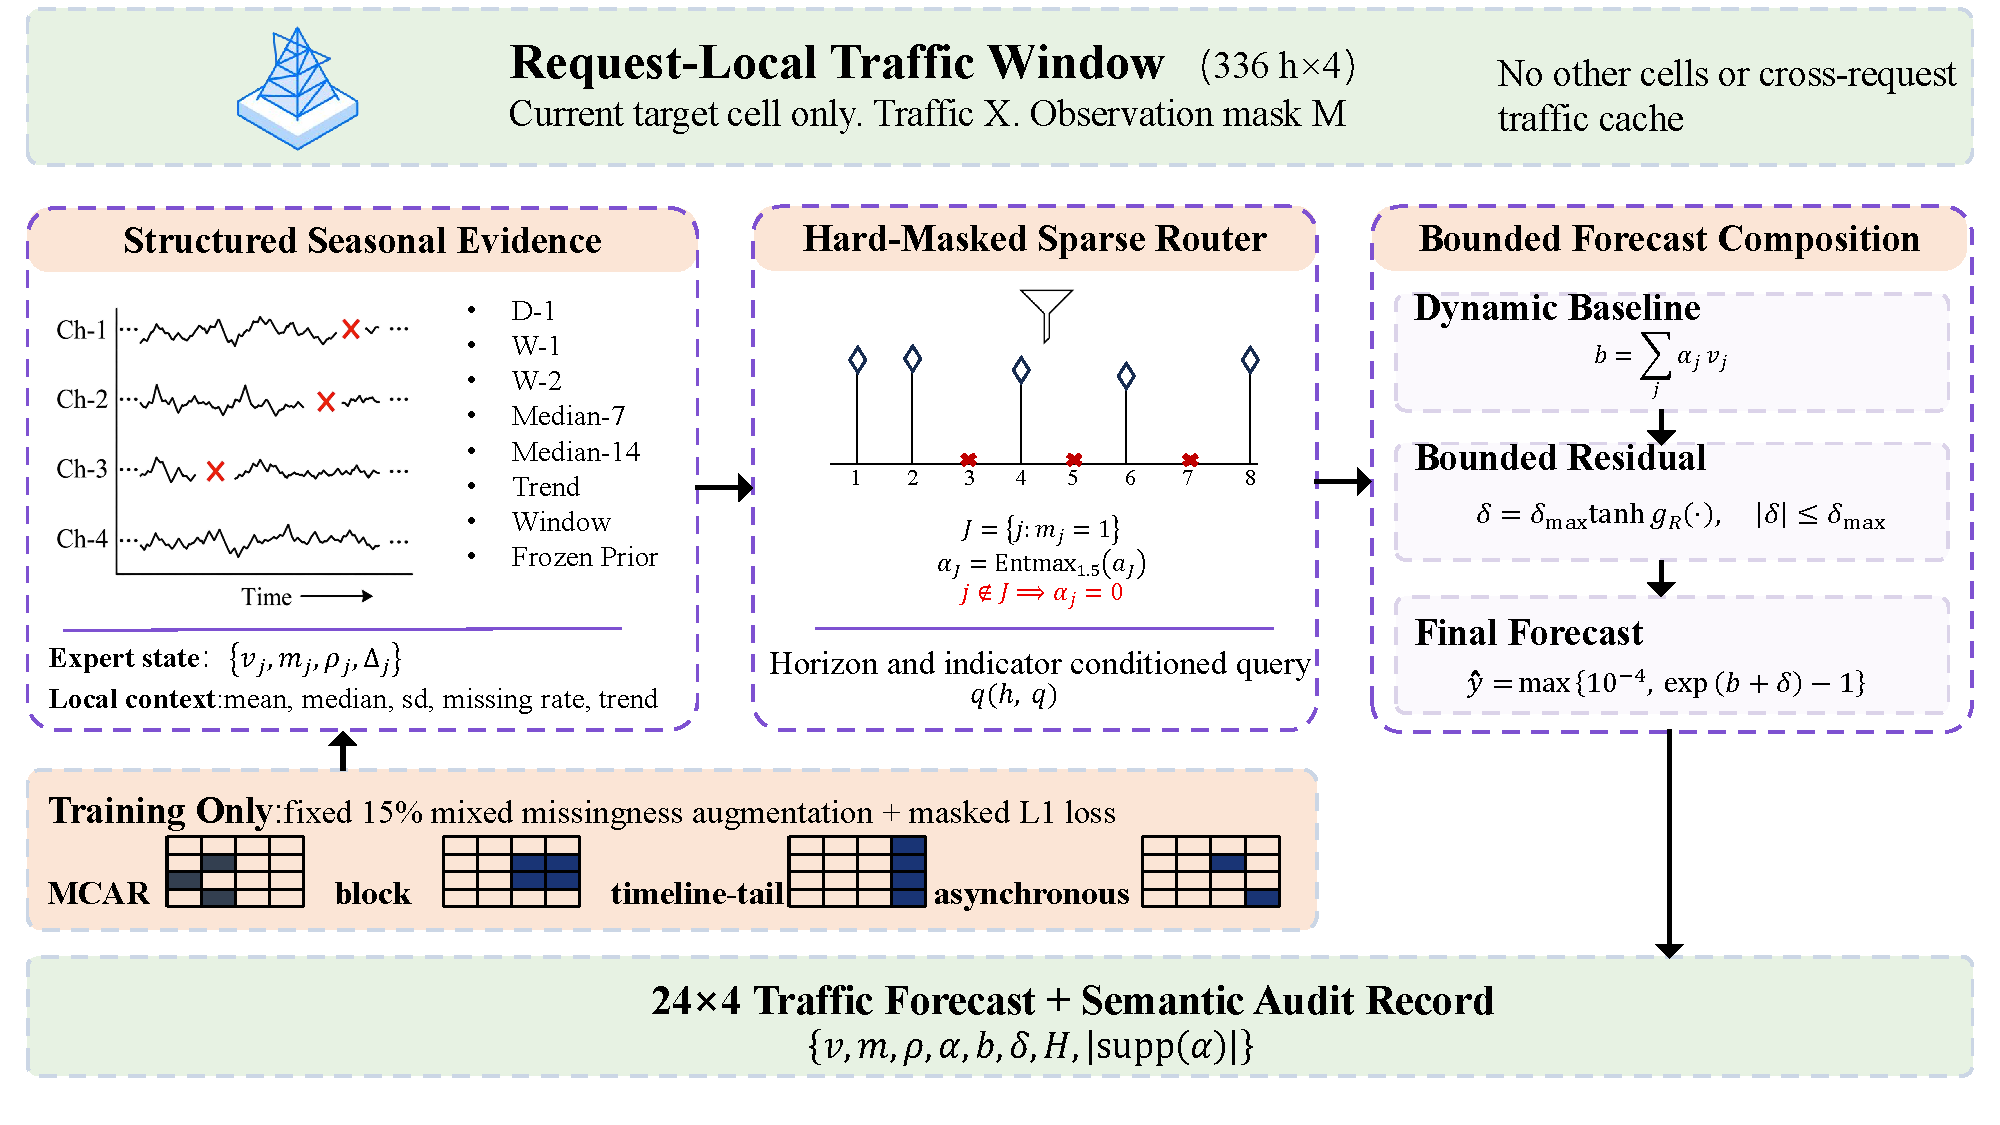
\includegraphics[width=\textwidth]{figures/fig_architecture.pdf}
\caption{\method{} as an instance of structured seasonal expert routing. One masked 336-hour request constructs a finite expert bank; horizon-conditioned routing hard-masks unavailable evidence and produces a dynamic baseline, bounded correction, $24\times4$ forecast, and core fields for a proposed audit record.}
\label{fig:architecture}
\end{figure*}

\section{Experimental Methodology}
\subsection{Data, split, and evidence status}
The anonymous trace contains 527,760 hourly records from 736 cells from July 20 to August 18, 2024. The panel is incomplete: 730 cells contain 720 hours and six contain 360 hours. Each indicator has 69,014 missing cell-hour values, or 13.08\% of the 527,760 cell-hour records; the observed mask is shared across the four indicators.

Daily sliding yields 11,686 candidate 336-to-24-hour windows. One window, cell 2062 at the August 4 origin, has a 25-hour discontinuity and is reported rather than repaired; 11,685 continuous windows remain. Targets on August 3--9 form the fit layer (5,115 windows), August 10--11 the inner layer (1,460), and August 12--18 the evaluation layer (5,110). All 730 long-series cells contribute seven evaluation windows. Per-cell WAPE is defined for 727 cells; three lack a positive evaluable denominator after target masking. The evaluation contains 122,640 forecast hours and 106,248 observed target hours per indicator.

The evaluation period was already examined in earlier iterations of this study. For the later GRU-D comparison, its candidate grid, inner-layer selection rule, augmentation view, five model seeds (42--46), corruption seeds (142--146), metrics, and bootstrap procedure were fixed before that comparison was executed and finally aggregated. These choices maintain a fixed protocol throughout execution and final aggregation.

\subsection{Baselines, fairness, and optimization}
Clean comparison includes same-hour median; \fixedmixture{}; learned global and horizon--indicator mixtures; a 165D Standard-stat LightGBM; the precisely aligned traffic-only \originalmethod{}; DLinear; PatchTST; GRU-D-Direct-Aug; and A1--A6 router variants. Exact alignment of \originalmethod{} covers all 122,640 forecast keys with no duplicates. Both tree baselines use LightGBM~\cite{ke2017lightgbm} with 48 leaves, minimum leaf size 80, learning rate 0.04, feature fraction 0.88, bagging fraction 0.90, $\lambda_1=0.05$, $\lambda_2=0.20$, and maximum bin 127. \originalmethod{} uses 73 traffic-only features and fixed target-specific rounds 341/332/742/678.

The primary robustness analysis uses a controlled augmentation-matched comparison between \method{} (A6), DLinear-Aug, PatchTST-Aug, and an adapted missing-aware GRU-D-Direct-Aug control. For each of five model seeds, all four models receive the same deterministic 15\% mixed input-history view and use the same fit dates, inner dates, and fit-plus-inner refit schedule. Selection is confined to the same inner dates but is model-family specific: WLCR-SEA minimizes inner macro-over-indicator WAPE, using fit-frozen THS as a tie-break, whereas the neural baselines maximize the inner mean of four MAPE hit rates recorded as MAPEAUC after an inner-derived fifth-percentile filter, using lower inner mean MAPE as a tie-break. Clean-trained DLinear and PatchTST are retained only to quantify the independent contribution of augmentation.

DLinear, PatchTST, and GRU-D-Direct-Aug normalize log1p inputs and targets using statistics from the applicable training layer---fit dates during candidate selection and fit-plus-inner dates during final refitting---and minimize masked L1 in \emph{normalized target space}; predictions are inverse-normalized before raw-scale evaluation. GRU-D-Direct-Aug computes post-corruption per-indicator elapsed time strictly within each 336-hour request: at its first hour, $\Delta_{1,q}=0$ when observed and $\Delta_{1,q}=1$ otherwise. If no earlier observation exists inside that request, its previous value is initialized to the applicable training-layer mean (zero in standardized space); no pre-window telemetry is queried. The model learns input and hidden-state decays, feeds $[\mathrm{imputed\ value},\mathrm{mask}]$ to a GRUCell, and maps the final hidden state directly to a $24\times4$ normalized-log forecast. Dropout 0.10 is applied only to this final hidden state immediately before the direct output head during training; no input or recurrent dropout is used.

In contrast, WLCR-SEA uses the unnormalized log1p domain for experts, prior, residual, and masked L1, preserving the fixed interpretation of $\kappa$, $\delta_{\max}$, and the audit envelope. All neural and routing models use AdamW, weight decay $10^{-4}$, at most 100 epochs, patience 10, and five model seeds. WLCR-SEA uses batch size 256, whereas DLinear, PatchTST, and GRU-D-Direct-Aug use batch size 128. DLinear candidates are kernel 25 with learning rate $10^{-3}$ and kernel 49 with learning rate $5\times10^{-4}$. PatchTST uses patch length 24 and stride 12; its candidates are $(d,\mathrm{heads},\mathrm{layers},\mathrm{FF},\mathrm{dropout})=(32,4,1,64,0.1)$ and $(48,4,2,96,0.1)$ at the corresponding learning rates. GRU-D-Direct-Aug candidates are hidden size 32 at learning rate $10^{-3}$ and hidden size 48 at learning rate $5\times10^{-4}$, both with the stated output-head dropout. Router candidates are $(d,\mathrm{hidden},\eta,\delta_{\max})=(16,32,10^{-3},0.25)$ or $(32,64,5\times10^{-4},0.5)$. Each model's configuration and epoch count are selected only on the inner dates using the model-family criterion stated above, followed by reinitialization and refitting on the fit-plus-inner dates.

For the five final GRU-D members, the inner layer selected hidden size 32 for seeds 42/43/45 at epochs 53/41/17 and hidden size 48 for seeds 44/46 at epochs 95/35. Selected best epochs therefore range from 17 to 95. The size-48 candidate for seed 44 ran through the 100-epoch cap, but its selected epoch was 95.

We report five deterministic cell-disjoint folds as a complementary single-model-seed (42) refit audit, not as a five-seed ensemble. For each neural or routing model, architecture, selected configuration, epoch count, and optimizer settings are frozen from its temporal seed-42 run. Every fold uses the matched final-refit input-history view from augmentation seed 100042; WLCR-SEA retains batch size 256, while DLinear-Aug and PatchTST-Aug retain batch size 128. Each outer fold refits only on complementary cells, with no fold-specific retuning; every evaluation cell is excluded from priors, normalizations, neural weights, router weights, and boosters.

\subsection{Metrics, ensembles, and uncertainty}
All reported WAPE, MASE, and sMAPE values are computed after inverse transformation on the raw traffic scale. The primary metric is macro-over-indicator WAPE:
\begin{equation}
\operatorname{WAPE}_{\mathrm{macro}}=
\frac14\sum_{q=1}^{4}
\frac{\sum_i|y_{i,q}-\widehat y_{i,q}|}{\sum_i|y_{i,q}|}.
\end{equation}
For request $i$ and indicator $q$, the request-local 168-hour MASE scale is
\begin{equation}
d_{i,q}=\frac{1}{|\mathcal P_{i,q}|}\sum_{u\in\mathcal P_{i,q}}
|x_{i,u,q}-x_{i,u-168,q}|,
\end{equation}
where $\mathcal P_{i,q}$ retains only finite history endpoint pairs. A request--indicator group contributes to MASE only if $\mathcal P_{i,q}$ is nonempty and $d_{i,q}>10^{-12}$; MASE averages the resulting scaled absolute errors. All 20,356 request--indicator groups with observed holdout targets (424,992 target values) are MASE eligible, so the measured coverage is 100\%. We define sMAPE as
\begin{equation}
\operatorname{sMAPE}=\frac{2|y-\widehat y|}{\max(|y|+|\widehat y|,10^{-12})}.
\end{equation}
We additionally report pooled WAPE and a threshold hit score (THS). THS averages strict hit rates at MAPE thresholds $\{0.2,0.3,0.4,0.5\}$ after applying fifth-percentile filters frozen from the applicable training layer. WLCR-SEA inner selection uses the fit dates; reported temporal holdout metrics use fit plus inner dates; and each cell-disjoint fold uses its complementary training cells. THS is not an area under a curve.

Unless explicitly marked as deterministic, tree-based, or single-member deployment results, all primary \emph{temporal} neural and routing accuracy results use arithmetic five-seed prediction ensembles. The cell-disjoint audit is reported separately and fixes one model seed (42). The deployment table separately reports each timed single-member or ensemble configuration. With model seed $s\in\{42,\ldots,46\}$ and corruption seed $r\in\{142,\ldots,146\}$,
\begin{equation}
\widehat y^{(r)}=\frac15\sum_s\widehat y^{(s,r)},\qquad
\bar W=\frac15\sum_r\operatorname{WAPE}(\widehat y^{(r)}).
\end{equation}
Paired 95\% intervals use 5,000 cell-cluster bootstrap replicates. Each replicate resamples cells, retains all of each sampled cell's dates and horizons, recomputes indicator-specific ratios of sums, and then averages the four indicator WAPEs. For corruption results, paired deltas are first averaged over corruption seeds within each bootstrap replicate. Primary paired comparisons match \method{} to DLinear-Aug, PatchTST-Aug, and GRU-D-Direct-Aug, while predecessor summaries are reported separately. Intervals are unadjusted descriptive estimates; the explicitly labeled RQ3 seed-level $t$-intervals summarize optimization-seed variation. For stochastic mechanisms, estimates are conditional on the five fixed masks from seeds 142--146. For the cell-disjoint audit, the same construction resamples 727 evaluable cells while keeping the five fold refits and their seed-42 predictions fixed. Those intervals describe cross-cell sampling variation conditional on the recorded refits; they do not include optimization-seed, augmentation-view, hyperparameter-selection, temporal-period, or regional uncertainty. The broader inferential scope is summarized in Discussion.

\subsection{Corruption protocol}
Robustness masks are generated on each cell's unique absolute timeline \emph{before} overlapping requests are extracted. Thus one real timestamp has one corruption state across all requests. The observed masks are synchronous across the four indicators; asynchronous loss provides a controlled stress mechanism. We evaluate MCAR, one contiguous block, the tail of the unique evaluated timeline (timeline-tail), and asynchronous per-indicator loss at requested rates $\{0.1,0.2,0.3,0.5\}$.

\noindent\textbf{Corruption procedure.} For each mechanism, requested rate, and corruption seed: (1) construct an outage mask on unique cell--time--indicator keys; (2) superimpose it on original missingness without changing target labels; (3) slice the corrupted timeline into the original overlapping requests; (4) refill each neural input only from observations remaining inside that request; and (5) report both unique-key missingness and repeated window-exposure missingness. Five seeds (142--146) are used for stochastic mechanisms, while timeline-tail is deterministic for a fixed rate. For \originalmethod{}, the same mask is injected before its native 73D feature construction; clean replay is verified against the aligned stored prediction before stress results are accepted.

At 50\% block corruption, window-exposure missingness reaches 67.28\% due to unequal timestamp repetition.

The five deterministic cell-disjoint folds cover all 5,110 evaluation windows with zero cell overlap under the single-seed protocol described above. Formal latency uses the same Intel Xeon E5-2686 v4 host, one CPU thread, batch size one, 256 request identities, 128 warm-ups, and 2,048 measurements. Five-member ensembles are executed serially on that thread, with preprocessing recomputed for each member before raw predictions are averaged. The benchmark covers request-local expert preprocessing, the model forward pass (including routing weights, baseline, residual, and entropy), inverse transformation, and output floor.

\section{Results}
\subsection{RQ1: What is gained on clean history?}
Table~\ref{tab:clean} reports clean accuracy, while Fig.~\ref{fig:accuracy} isolates the routing hierarchy. \fixedmixture{} is distinct from \originalmethod{}: the latter reaches 0.1951 WAPE, whereas \method{} reaches 0.1955, with paired difference $+0.00045$ and 95\% CI $[-0.00312,0.00366]$. The interval includes zero, so this unadjusted analysis did not detect a clean-data difference; the point estimate for \method{} is marginally higher.

Second, learned static controls locate the fixed-to-dynamic improvement. Global indicator weights obtain 0.2048, horizon--indicator weights 0.2020, dynamic Softmax 0.1972, and dynamic Entmax (A2) 0.1964. The hard-masked A3 variant obtains 0.1967; it enforces the access policy by assigning unavailable experts exactly zero mass. Most of the fixed-to-learned improvement comes from learning indicator-specific mixture weights, with horizon conditioning and request context providing smaller additional gains.

The clean ranking favors DLinear at 0.1854. The adapted dedicated missing-aware GRU-D-Direct-Aug control obtains 0.2235 WAPE, with individual complete-target macro WAPEs of $0.2287\pm0.0124$ (mean $\pm$ sample SD across five seeds). \method{} minus DLinear is $+0.01007$ (CI $[0.00696,0.01395]$), and versus PatchTST it is $+0.00399$ (CI $[0.00038,0.00743]$). Conversely, \method{} improves Standard-stat LightGBM by $-0.02167$ (CI $[-0.02712,-0.01618]$). Mixed augmentation slightly worsens clean DLinear and PatchTST, quantifying the cost of robustness training on clean data.

\begin{table*}[t]
\centering
\caption{Clean evaluation under matched request-local information. \emph{Aug.} denotes the same 15\% mixed input-history augmentation used by \method{} (A6), DLinear-Aug, PatchTST-Aug, and GRU-D-Direct-Aug. Neural and routing rows are five-seed ensembles; deterministic and LightGBM rows are single fitted models. Lower error is better; higher THS is better.}
\label{tab:clean}
\footnotesize
\setlength{\tabcolsep}{4.8pt}
\begin{tabular}{>{\raggedright\arraybackslash}p{0.31\textwidth}lcccc}
\toprule
Method & Training view & WAPE & MASE & sMAPE & THS\\
\midrule
\fixedmixture{} & deterministic & 0.2368 & 0.9408 & 0.2791 & 0.7095\\
Learned global indicator weights & clean & 0.2048 & 0.8473 & 0.2519 & 0.7627\\
Learned horizon--indicator weights & clean & 0.2020 & 0.8255 & 0.2469 & 0.7688\\
Standard-stat LightGBM & clean & 0.2172 & 0.8802 & 0.2605 & 0.7438\\
\originalmethod{} & clean & 0.1951 & 0.7848 & 0.2382 & 0.7822\\
DLinear & clean & \textbf{0.1854} & \textbf{0.7719} & \textbf{0.2343} & 0.7884\\
DLinear-Aug & mixed 15\% & 0.1907 & 0.7877 & 0.2454 & 0.7789\\
PatchTST & clean & 0.1915 & 0.7826 & 0.2369 & \textbf{0.7909}\\
PatchTST-Aug & mixed 15\% & 0.1960 & 0.7999 & 0.2434 & 0.7855\\
GRU-D-Direct-Aug & mixed 15\% & 0.2235 & 0.9076 & 0.2675 & 0.7337\\
\method{} (A6) & mixed 15\% & 0.1955 & 0.7906 & 0.2401 & 0.7816\\
\bottomrule
\end{tabular}
\end{table*}

\begin{figure}[t]
\centering
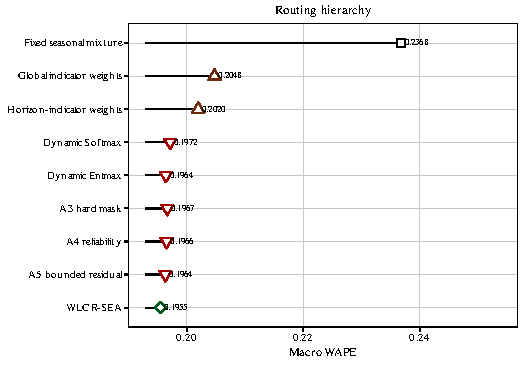
\includegraphics[width=\columnwidth]{figures/wlcr_sea_clean_accuracy.pdf}
\caption{Routing hierarchy on the clean holdout. Indicator-specific weights account for most of the fixed-to-learned improvement.}
\label{fig:accuracy}
\end{figure}

\subsection{RQ2: Does the method remain robust under an augmentation-matched protocol?}
Figure~\ref{fig:missingness} presents the predecessor stress profile in panel~(a) and the augmentation-matched paired comparisons in panel~(b) and Table~\ref{tab:robust-ci}. The matched controls are DLinear-Aug, PatchTST-Aug, and GRU-D-Direct-Aug.

At 20\% block and timeline-tail loss, and at 30\% asynchronous loss, \method{} records WAPE 0.2017, 0.2048, and 0.2045, respectively. Its paired intervals versus DLinear-Aug and PatchTST-Aug span zero in all six comparisons, whereas all three listed GRU-D-Direct-Aug intervals lie below zero. At 50\% requested corruption, \method{} records WAPE 0.2196 for block loss, 0.2460 for timeline-tail loss, and 0.2172 for asynchronous loss; all nine listed augmentation-matched intervals lie below zero.

At 50\% corruption, \originalmethod{} obtains macro WAPE 0.2636/0.3234/0.2261 under block/timeline-tail/asynchronous masks, versus 0.2196/0.2460/0.2172 for \method{}. This predecessor stress profile is reported separately from the augmentation-matched comparison.

\begin{table*}[t]
\centering
\caption{Paired five-seed-ensemble robustness results. Entries are the \method{} minus baseline WAPE difference with 5,000 unadjusted paired cell-cluster-bootstrap 95\% intervals; negative favors \method{}. Matched baselines are exactly DLinear-Aug, PatchTST-Aug, and GRU-D-Direct-Aug; \originalmethod{} is excluded from this table. For stochastic mechanisms, intervals are conditional on five fixed corruption-mask realizations.}
\label{tab:robust-ci}
\footnotesize
\setlength{\tabcolsep}{3.0pt}
\begin{tabular}{lcccc}
\toprule
Condition & \method{} WAPE & \shortstack{$\Delta$ vs.\\DLinear-Aug [95\% CI]} & \shortstack{$\Delta$ vs.\\PatchTST-Aug [95\% CI]} & \shortstack{$\Delta$ vs.\\GRU-D-Direct-Aug [95\% CI]}\\
\midrule
20\% block & 0.2017 & $-0.00030$ [$-0.00308$, $0.00259$] & $-0.00030$ [$-0.00379$, $0.00278$] & $-0.03339$ [$-0.04052$, $-0.02619$]\\
20\% timeline-tail & 0.2048 & $-0.00150$ [$-0.00407$, $0.00115$] & $-0.00168$ [$-0.00541$, $0.00182$] & $-0.05270$ [$-0.06220$, $-0.04297$]\\
30\% asynchronous & 0.2045 & $-0.00175$ [$-0.00465$, $0.00124$] & $-0.00162$ [$-0.00531$, $0.00192$] & $-0.02597$ [$-0.03323$, $-0.01820$]\\
50\% block & 0.2196 & $-0.04022$ [$-0.04562$, $-0.03500$] & $-0.02050$ [$-0.02496$, $-0.01603$] & $-0.04953$ [$-0.05590$, $-0.04317$]\\
50\% timeline-tail & 0.2460 & $-0.03451$ [$-0.04304$, $-0.02669$] & $-0.01569$ [$-0.02292$, $-0.00899$] & $-0.06970$ [$-0.08060$, $-0.05871$]\\
50\% asynchronous & 0.2172 & $-0.02044$ [$-0.02426$, $-0.01657$] & $-0.01303$ [$-0.01701$, $-0.00913$] & $-0.03504$ [$-0.04215$, $-0.02771$]\\
\bottomrule
\end{tabular}
\end{table*}

\begin{figure*}[t]
\centering
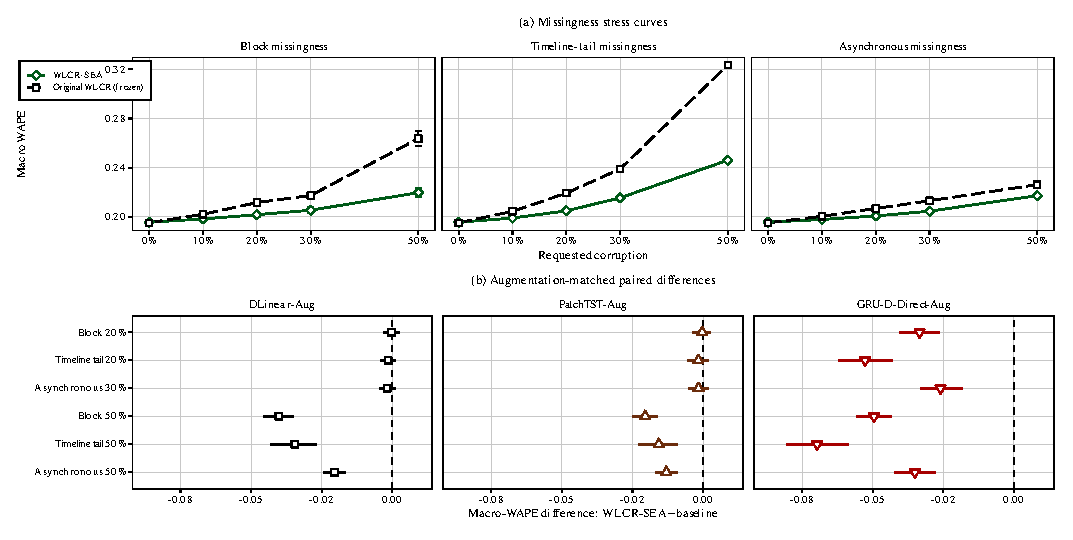
\includegraphics[width=\textwidth]{figures/wlcr_sea_missingness.pdf}
\caption{Missingness robustness. (a) \method{} and \originalmethod{} under five fixed masks; the predecessor curve is reported separately from the augmentation-matched comparison. (b) Unadjusted paired 95\% intervals versus augmentation-matched neural controls; negative favors \method{}.}
\label{fig:missingness}
\end{figure*}
\begin{table*}[!t]
\centering
\caption{One-thread, batch-one prediction-only deployment cost, including preprocessing and inverse transformation/output floor. Five-member ensembles are serial. KiB uses 1,024 bytes and covers checkpoint and frozen-model assets, not proposed audit payloads. Clean WAPE is reported for timed deployments. GRU-D-Direct-Aug was not included in this CPU protocol; ``not measured'' and ``--'' denote unavailable comparable latency and audited deployment-asset size, not zero cost.}
\label{tab:latency}
\footnotesize
\setlength{\tabcolsep}{4.0pt}
\begin{tabular}{llrrrrr}
\toprule
Family & Deployment & WAPE & P50 (ms) & P95 (ms) & P99 (ms) & KiB\\
\midrule
\method{} & single seed (42) & 0.1959 & 6.802 & 7.301 & 7.574 & 16.2\\
\method{} & five-seed ensemble & 0.1955 & 34.705 & 37.420 & 38.684 & 148.8\\
DLinear-Aug & single seed (42) & 0.1936 & \textbf{0.506} & \textbf{0.558} & \textbf{0.576} & 67.1\\
DLinear-Aug & five-seed ensemble & 0.1907 & 2.402 & 2.530 & 2.564 & 335.4\\
PatchTST-Aug & single seed (42) & 0.1998 & 1.087 & 1.149 & 1.179 & 143.6\\
PatchTST-Aug & five-seed ensemble & 0.1960 & 7.270 & 7.482 & 7.592 & 1,057.1\\
GRU-D-Direct-Aug & five-seed ensemble & 0.2235 & \multicolumn{3}{c}{not measured} & --\\
\originalmethod{} & traffic-only 73D, single seed (42) & 0.1951 & 13.290 & 14.344 & 15.425 & 9,316.8\\
\bottomrule
\end{tabular}
\end{table*}

Table~\ref{tab:variants} separates the A3--A6 mechanisms. Their clean WAPEs are 0.1967, 0.1966, 0.1964, and 0.1955, respectively. The A4--A3 point difference remains small after reliability is removed from every A1--A3 input and loss path. Reliability therefore serves as an inspectable support descriptor, while the bounded residual gives a small clean point improvement and the primary severe-loss advantage is associated with mixed augmentation.

\subsection{RQ3: Which audit claims survive direct tests?}
The structural checks pass exactly. Across five model seeds, maximum unavailable-expert weight is 0, and all bounded-envelope checks have zero maximum violation. Effective support is $5.223$ experts on average; the five independently trained members yield a 95\% seed-level $t$-interval of $[5.101,5.345]$. Thus, sparsity here means exact zeros rather than one-expert routing. The residual remains small relative to the baseline for most forecasts: the five-seed mean P50/P90 ratios are 0.00615/0.03068.

The implementation-level locality test deterministically stratifies 256 target requests across 253 cells, all seven evaluation dates, and four missingness bins. For each target, it perturbs every non-target pre-extracted request object, including same-cell non-target objects, while preserving the target object. Expert values, masks, reliabilities, context, attention, baseline, residual, entropy, and prediction remain bitwise identical in all 256 tests ($N_{\mathrm{violations}}=0$). This establishes request-object-level invariance of the serving path under the recorded field allowlist.

Deletion is recomputed rather than approximated by cached-weight renormalization: the selected available non-prior expert is hard-masked, its reliability is set to zero, and attention and residual are rerun. On the five-seed ensemble, top-weight deletion increases macro WAPE by 0.00595 (cell-cluster-bootstrap CI $[0.00441,0.00757]$), versus 0.00104 ($[0.00079,0.00131]$) for expected matched-random deletion (10 repeats per model seed). Across the five member models, the mean per-member Spearman correlation between expert weight and leave-one-out prediction influence is 0.693 (95\% seed-level $t$-interval $[0.678,0.708]$). These deletion results support behavioral relevance under the recorded audit.

By contrast, the five per-member entropy--APE Spearman correlations have mean $-0.0196$ (95\% seed-level $t$-interval $[-0.0407,0.0016]$), so attention entropy is not used as an uncertainty estimate. Figure~\ref{fig:audit} consolidates these findings.

\begin{figure*}[t]
\centering
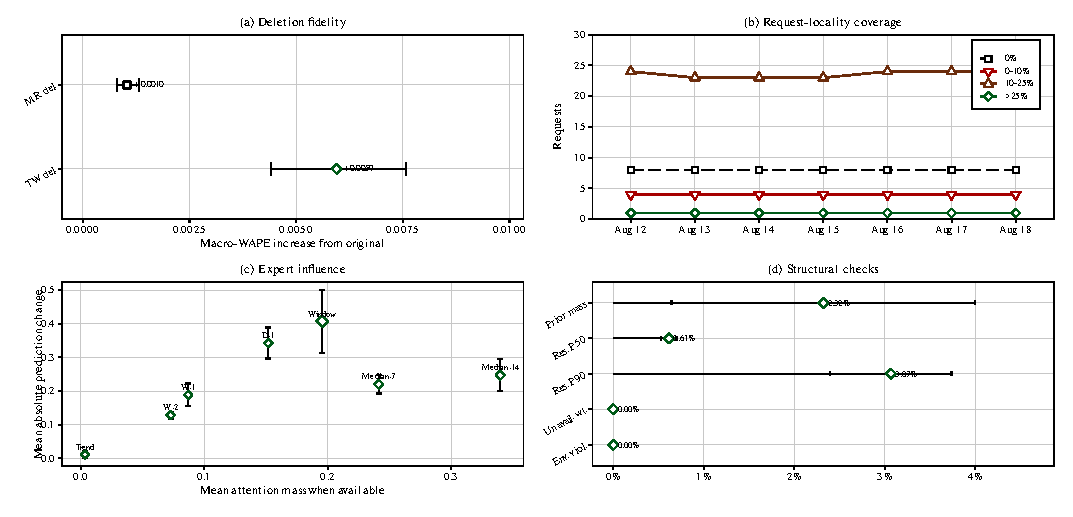
\includegraphics[width=\textwidth]{figures/wlcr_sea_auditability.pdf}
\caption{Auditability evidence: rerouted deletion, expert influence, structural checks, and zero-violation locality coverage over 256 requests. Axis labels in (a,d): TW, top-weight; MR, matched-random; del., deletion; Res., residual; wt., weight; Unavail., unavailable; Env., envelope; Prior mass, mean prior mass.}
\label{fig:audit}
\end{figure*}
\subsection{RQ4: What is observed under cell-disjoint refitting, and at what deployment cost?}
The five deterministic cell-disjoint folds exclude evaluation cells from every fold-fitted quantity and cover all \RQFourEvaluationWindowCount{} windows with zero cell overlap. Under the protocol-matched single-model-seed (\RQFourModelSeed{}) refits, \method{} obtains \RQFourWLCRWAPE{} WAPE versus \RQFourDLinearWAPE{} for DLinear-Aug; the paired difference is $\RQFourDLinearDelta{}$, with an unadjusted 95\% cell-cluster-bootstrap interval of $[\RQFourDLinearCILow{},\RQFourDLinearCIHigh{}]$. Against \originalmethod{} (\RQFourOriginalWAPE{}), the difference is $\RQFourOriginalDelta{}$ with interval $[\RQFourOriginalCILow{},\RQFourOriginalCIHigh{}]$; against PatchTST-Aug (\RQFourPatchWAPE{}), it is $\RQFourPatchDelta{}$ with interval $[\RQFourPatchCILow{},\RQFourPatchCIHigh{}]$. Point WAPEs for Same-hour median and \fixedmixture{} are \RQFourSameHourWAPE{} and \RQFourFixedMixtureWAPE{}, respectively. These descriptive intervals resample \RQFourClusterCount{} cells and are conditional on the fixed seed-\RQFourModelSeed{} refits; they do not quantify optimization-seed or protocol-selection uncertainty. Mean unseen-cell prior mass is \RQFourPriorMassPercent{}\% across folds.

Table~\ref{tab:latency} pairs each timed prediction-only deployment with its own clean WAPE. The main accuracy result is the five-seed ensemble, so its 34.70/38.68 ms P50/P99 latency and 148.8 KiB checkpoint and frozen-model assets are the deployment-aligned values. Five members execute serially on the same one-thread setting, with preprocessing recomputed for each member. The table reports prediction-only inference, from request-local preprocessing through inverse transformation and output flooring. DLinear and PatchTST remain faster, while the traffic-only \originalmethod{} is larger and slower than a single \method{} member.



\section{Discussion}\label{sec:discussion}
The expert bank is manually specified and favors periodic behavior; sudden events without local precedents can be missed. Entmax creates exact zeros, but most forecasts still use about five experts. The reliability descriptor has no independent performance evidence in the corrected ablation, and the bounded residual can hurt robustness without augmentation. These modules should not be presented as equal sources of gain.

The current trace covers one anonymous region and roughly one month. All origins are midnight, so horizon and clock hour are confounded; additional origins, seasons, and regions are required to assess external generalization. The August holdout informed the redesign, so the current evaluation is exploratory pending validation on a prospectively untouched period. The cell-disjoint analysis is a within-trace exclusion audit rather than evidence of cross-region generalization. It fixes one model seed (42), uses one matched deterministic final-refit augmentation view, and performs no fold-specific or nested retuning. Its cluster-bootstrap intervals resample 727 observed cells conditional on those fixed refits and therefore do not capture retraining, hyperparameter-selection, temporal, or regional uncertainty. An interval below zero is consequently a directional result for the recorded comparison, not evidence of model-family-wide superiority.

GRU-D-Direct-Aug provides a dedicated missing-aware direct-forecasting control, and the predecessor stress profile is reported separately from augmentation-matched comparisons. Paired intervals are unadjusted descriptive estimates conditioned on five fixed corruption-mask realizations; they characterize cross-cell uncertainty rather than family-wise effects across model families, mechanisms, rates, indicators, and audit tests. The corruption mechanisms preserve absolute-timeline consistency across requests. Five-seed ensembling improves reported accuracy and multiplies serving cost; Table~\ref{tab:latency} reports both ensemble and single-member deployments.

Request-object serving-path invariance is verified as an implementation property under the recorded allowlist; upstream request construction remains outside this test. The serving path is not a privacy guarantee because global parameters and the frozen prior capture training-distribution information. Attention and deletion analyses characterize behavioral relevance, while entropy does not provide a useful uncertainty estimate. Future extensions can incorporate weather, coordinates, static parameters, provisioning, and operational scheduling where they are available to the scoring path.

The serving policy models a self-contained online scoring path. Future work can quantify the availability, latency, and fault-containment properties of ingress--scoring separation, and compare this interface with graph models supplied with authorized neighbor states. Such evaluations will map the conditions in which request-local and richer spatial evidence provide complementary value.

\section{Conclusion}
Structured seasonal expert routing turns a fixed request-local mixture into a horizon-conditioned, available-set-masked, and bounded prediction path with core fields for a proposed fixed-schema semantic audit record. On clean history, the unadjusted paired interval for \method{} versus \originalmethod{} includes zero, so this analysis does not detect a difference; DLinear has the lowest clean WAPE. Under matched augmentation, the selected moderate-loss intervals versus DLinear-Aug and PatchTST-Aug include zero, whereas at the listed 50\% structured-corruption conditions all nine differences versus the three augmentation-matched baselines are negative with intervals below zero, conditional on five fixed masks. Recorded implementation checks yield zero unavailable-expert mass, zero bounded-envelope violations, and bitwise serving-path invariance across 256 stratified request-object tests under the field allowlist. Under the protocol-matched single-seed cell-disjoint refits, the intervals versus DLinear-Aug and \originalmethod{} include zero, whereas the interval versus PatchTST-Aug lies below zero. Because these intervals condition on fixed refits, they do not establish retraining or cross-region generalization. The present evidence therefore identifies an exploratory robustness--inspectability--cost profile for request-local serving. Prospective validation on longer, cross-region, and cross-season data, together with comparisons using authorized neighbor information, is required to determine how this profile generalizes.

\section*{Code and Data Availability}
The implementation is open source at
\url{https://github.com/rudykon/WLCR-SEA_Predictor}.
Information on obtaining the data used in this study may also be consulted at the same link.

\bibliographystyle{IEEEtran}
\bibliography{references}

\end{document}
